\documentclass[12pt]{article}

\usepackage{amsmath}
\usepackage{physics}
\usepackage{mhchem}
\usepackage[labelfont=bf]{caption}
\usepackage{graphicx}
\usepackage{comment}
\usepackage{color, soul}    % for text highlighting
\usepackage{float}          % for more controlled placement of figures in text

\usepackage[style=phys]{biblatex}       % citations!
\addbibresource{main.bib}

% Defines the subfigure environment
\usepackage{subcaption}

% Puts the abstract on the title page
\usepackage{titling}
\newsavebox{\abstractbox}
\renewenvironment{abstract}
 {%
  \global\setbox\abstractbox=\vtop\bgroup
  \begin{center}\bfseries\abstractname\end{center}%
 }
 {\par\egroup}
\renewcommand{\maketitlehookd}{%
  \par\vfil
  \box\abstractbox
}

%% Not sure what this does when changing document type to article
% Changes the formatting of the chapter numbers
\usepackage{titlesec}
% \titleformat{\chapter}
%   {\normalfont\LARGE\bfseries}{\thechapter}{1em}{}
% \titlespacing*{\chapter}{0pt}{3.5ex plus 1ex minus .2ex}{2.3ex plus .2ex}
\renewcommand{\sectionbreak}{\clearpage}


% TITLE DATA
\title{Development of a Visible Photoluminescence Microspectrometer}
\author{Zach Colbert}
\date{Spring 2019}


% For comments, notes, todos, etc.
\newcommand{\printnote}[2]{\hl{[\textbf{#1: #2}]}}
\newcommand{\todo}[1]{\printnote{TODO}{#1}}
\newcommand{\note}[1]{\printnote{NOTE}{#1}}

% Requested formatting from Minot, 3/20
\usepackage{geometry}
\geometry{letterpaper, margin=1in}
\linespread{1.6}

\begin{document}
  % TITLE PAGE
  % \begin{titlingpage}
    % \begin{abstract}
      % This is the abstract. It comes later.
    % \end{abstract}
    % \maketitle
  % \end{titlingpage}

  \begin{titlepage}
    \begin{center}
        \vspace*{1cm}
  
        \textbf{Development of a Visible Photoluminescence Microspectrometer}
  
        \vspace{3cm}
  
        % by \\
        \textbf{Zachary Colbert}
  
        \vspace{10cm}
  
        An undergraduate thesis advised by Matt W. Graham \\
        submitted to the Department of Physics, Oregon State University \\
        in partial fulfillment of the requirements for the degree of BSc in Physics
  
        \vfill
  
        % Presented X June 2020 \\
        Draft submitted on \today
  
    \end{center}
  \end{titlepage}

  \thispagestyle{plain}
\begin{center}
    % {\Large\textbf{Development of a Visible-NIR Photoluminescence Microspectrometer}}
 
    % \vspace{0.4cm}
    % by \\
    % \textbf{Zachary Colbert}
 
    % \vspace{0.9cm}
    \textbf{Abstract}
\end{center}

Photoluminescence (PL) is the process by which light is absorbed and re-emitted by a material. In solid-state physics, PL is an important characteristic measurement for studying the electron band structure of materials. Here we report the design and construction of a simple instrument which can accurately measure PL in thin-film materials on a micron spatial scale. We accomplish this by coupling a diode laser system to a metallurgical microscope, using optical filters to block light reflected by the sample. The instrument is equipped with a digital camera for imaging, and a commercial spectrometer for measuring PL spectra. We demonstrate the effectiveness of the instrument on thin-film samples of crystalline anthradithiophene and cadmium selenide quantum dots.

% FEEDBACK FROM CLASS: Very readable, terms understandable. Include more details about
% results: how do we determine that the measurements are good?
% Add future work notes

  \tableofcontents
  \listoffigures


  \section{Introduction}
  % \section{The Need for a Simpler Spectrometer (Motivation)}

Photoluminescence (PL) is the process by which materials will absorb a photon, exciting an electron to a higher-energy "excited state," then emit a photon as the electron relaxes back to a lower-energy state. Measuring PL in different ways is a common method for characterizing semiconducting materials.

Basic PL measurements are emission and excitation, and differ by their independent variables. Emission measurements use one wavelength to excite the material, and measure the intensity of light emitted across a chosen spectrum. Excitation measurements use many wavelengths to excite the material, and measure the intensity of light emitted at a particular wavelength. This project is centered around PL emission measurements.

The Micro-Femto Energetics ($\mu fE$) group at Oregon State University uses advanced optoelectronic methods to characterize materials, especially thin-layer materials and micron-scale semiconducting devices.

The group's workhorse when it comes to PL measurements is a Horiba \textbf{Something?} fluorimeter, coupled to a \todo{model?} microscope. The instrument uses a \todo{specs?} xenon-arc lamp and double-monochromator to illuminate a wide field with a tunable wavelength. The light source is coupled to the microscope with a fiber optic cable. The instrument can be configured for reflection or transmission microscopy depending on the application. With the aid of computer software, the instrument is able to measure both PL emission and excitation. However, there are a few distinct challenges to using this instrument.

Because the fiber optic delivers a large beam, a large area on samples is illuminated whether the instrument is in a reflection or transmission mode. The wide-field illumination is excellent for imaging, but makes it hard to isolate emissions from small spatial domains.

\todo{Something about the system takes a long time to warmup before the light source is stable.}

\todo{Check specs for monochromator. What is it's spectrum like vs. laser diode? More or less monochromatic?}

\todo{Something about training time and the learning curve for using the device. Software is kinda complicated. Takes a really long time to take a measurement.}

This project offers a solution to these challenges by designing and assembling a new PL microspectrometer that can measure the PL emission of samples accurately, quickly, and with the ability to illuminate small spatial domains.

Naturally, the new instrument has fewer applications. It only measures emission (not excitation), and reconfiguration for other measurements requires more consideration to optical design. The goal of this project, however, is to design an instrument that is simple to use for PL measurement when use of the fluorimeter is impractical, too time consuming, or the instrument is in use for another experiment.


  \section{Background}
  \subsection{Optoelectronic Materials}\label{chap:intro-optomats}

Optoelectronic materials convert light to electric energy and/or electric energy to light. The study of these materials goes back as far as the early 1900s, but accelerated rapidly in the 1960s with the advent of the light emitting diode and semiconductor laser \cite{sweeney_optoelectronic_2017}. Optoelectronic devices are ubiquitous; they have enabled the rapid growth of information technologies around the world, and are fundamental in modern telecommunication and internet infrastructure. Modern optronics research explores new materials that can be used to create faster, more efficient, and smaller optoelectronic devices.

\subsubsection{Organic Photovoltaic: ADT}\label{chap:intro-optomats-adt}

Organic optoelectronic materials are not a new discovery; however, they have become increasingly popular in recent decades as methods for creating them have advanced \cite{ostroverkhova_organic_2016}. The Ostroverkhova group at Oregon State University has studied several organic photovoltaics (OPVs) including functionalized derivatives of pentacene, benzothiophene, and anthradithiophene (ADT) \cite{e._b._shepherd_effect_2011, platt_optical_2009}. A drop-cast sample of fluorinated ADT with triethylsilyethynyl (TES) functional group, provided by the Ostroverkhova group, is used for demonstration of the new microspectrometer device in Chapter \ref{chap:results}.

\begin{figure}[H]
    \centering
    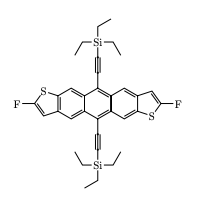
\includegraphics{img/adt-tes-f.png}
    \caption[Molecular diagram of ADT TES-F.]{Molecular diagram of fluorinated anthradithiophene (ADT) with triethylsilyethynyl (TES) side group. A drop-cast sample of this molecule was provided by the Ostroverkhova group at Oregon State University, and used for demonstration of our microspectrometer instrument following a study by Lam \cite{lam_polarization_2018}.}
    \label{fig:adt-diagram}
\end{figure}

\subsubsection{Quantum Dots: \ce{CdSe}}\label{chap:intro-optomats-qd}

Quantum dots (QDs) are artificial semiconductor particles, typically only a few nanometers in size. There has been a fair amount of research on the tunability of optoelectronic properties in QDs by varying their size and shape. Quantum dots have many of the same potential applications as other optoelectronic materials but are attractive for their size and reproducibility. Previous studies have shown how quantum dots can be produced en masse with a high degree of control over their shape and size \cite{empedocles_photoluminescence_1996, murray_synthesis_2000}.

A sample of CdSe quantum dots, suspended in solution and drop-cast on a glass slide, is used to demonstrate the new microspectrometer device in Chapter \ref{chap:results}.

\subsection{Mechanics of Photoluminescence}
Photoluminescence occurs in molecules where the valence and conduction bands are separated by a small band gap near the Fermi level. A molecule absorbs a photon with energy greater than or equal to its band gap, exciting an electron from its ground state in the valence band to an excited state in the conduction band. The electron lives in this excited state for a short time, and then relaxes back to the ground state.

The electron can relax non-radiatively --- losing energy as it transitions through vibrational modes --- or radiatively, losing a small amount of energy to vibrational transitions and then returning to the ground state. When it returns to the ground state, the energy is emitted as a photon. We expect the energy of this photon to be lower than that of the absorbed photon (and the wavelength longer) because of the loss of energy to vibrational transitions.

% Because of the loss of energy to vibrational transitions, we expect the energy of this photon to be lower than that of the absorbed photon, and the wavelength longer.

Measurement of fluorescent emissions yields information about the energy of these electron transitions, allowing us to map out the electron band structure of molecules.


  \section{Methods}
  \subsection{Design}

\subsubsection{Microscope}

The starting point of the project was an Olympus BX60M fluorescence microscope. The BX60M is built for reflection microscopy, and includes a housing for brightfield and darkfield mirrors. For the new instrument, we added a mirror cube housing between the brightfield/darkfield mirror housing and the observation tube. This additional component housed a dichroic mirror, which enabled us to couple an external light source into the instrument and filter that light out of the path through the observation tube.

\begin{figure}[H]
    \centering
    \includegraphics[width=0.5\textwidth]{img/microscope.png}
    \caption[Front view of microspectrometer instrument.]{Front view of microspectrometer instrument (laser controllers not pictured) built around Olympus BX60M fluorescence microscope. The laser diode mount and mirrors are shown on the left. Digital camera for sample imaging is mounted to the microscope eyepiece. We have mounted a collimating mirror to the observation tube (at the top of the microscope), which collects emissions and transmits them into a USB spectrometer via optical fiber.}
    \label{img:microscope}
\end{figure}


\subsubsection{Laser Excitation}
The BX60M is equipped with a xenon arc lamp, which is used for general observations under white light illumination. In order to measure photoluminescence, we require the use of a (mostly) monochromatic light source which is energetic enough to excite electrons in the sample.

\begin{figure}[h]
    \centering
    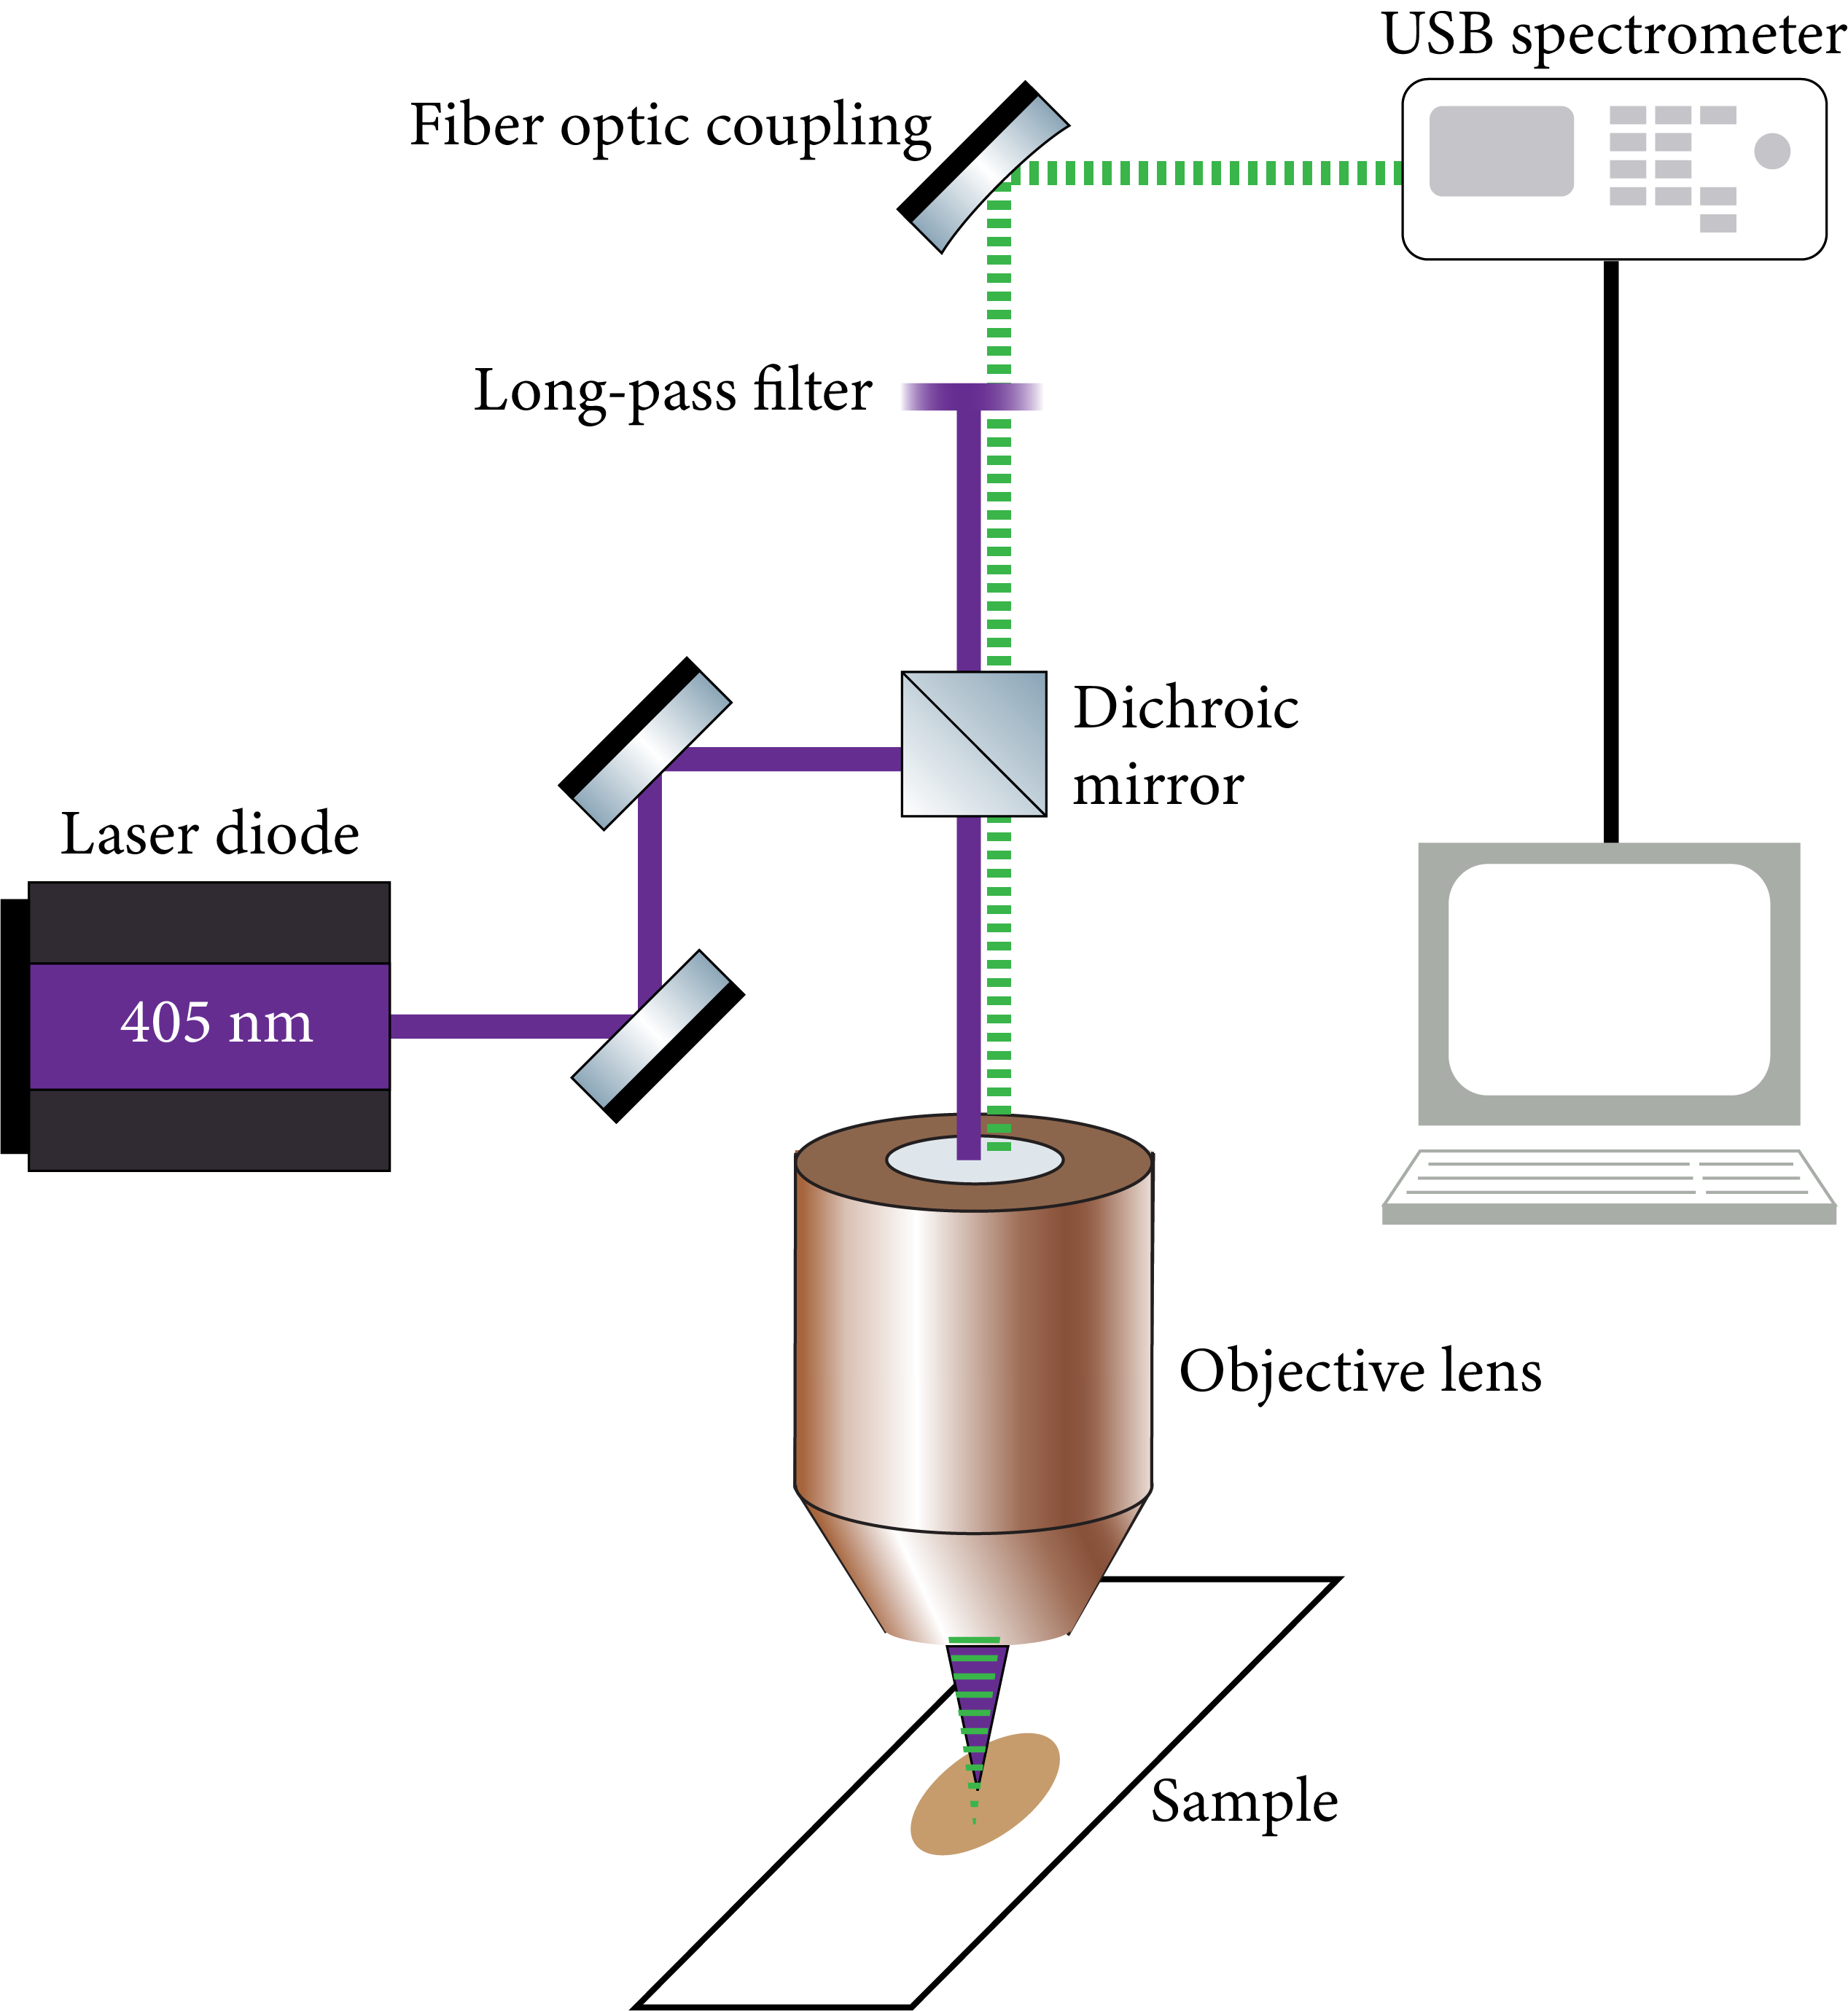
\includegraphics[width=.75\textwidth]{img/optical-diagram.png}
    \caption{Schematic diagram of the microspectrometer instrument.}
    \label{img:optical-diagram}
\end{figure}

Our instrument uses a diode laser as its light source. Specifically, we used a ThorLabs L405P20 laser diode (405 nm), TCLDM9 thermoelectrically-cooled mount, LDC 202 laser diode controller, and TED 200 temperature controller. To couple the laser and microscope, we used a set of two mirrors in a vertical beam fold configuration. \hl{This enabled precise alignment of the laser to the optical axis of the microscope, which maximizes transmission of excitation light through the objective lens and onto the sample stage.}

The laser diode housing and first mirror were mounted to an optical table. The laser starts parallel to the surface of the table, and the first mirror directs the beam upward. The second mirror in the beam fold was mounted to the end of a tube that extends out the side of the mirror cube housing. This mirror directs the vertical beam horizontally into the mirror. It seems preferable to mount both mirrors to the optical table for stability, but we were successful with this method by mounting the microscope to the table so that it and the second mirror did not move relative to the laser beam during normal operation.

\begin{figure}[H]
    \centering
    \includegraphics[width=0.5\textwidth]{img/microscope-side.png}
    \caption[Side view of microspectrometer instrument.]{Side view of microspectrometer instrument. Laser controllers are shown in the foreground. Between the controllers and the microscope, two flat mirrors and a dichroic mirror (not visible here) couple the laser light into the microscope's optical path.}
    \label{img:microscope-side}
\end{figure}

Due to limited space on the optical table, it was not feasible to align the laser diode housing and mirror cube housing in the plane of the table. To overcome this, our beam fold configuration also turns the beam 90 degrees in the plane of the table. The configuration we used has the laser beam initially pointed in the direction of the operator, then directed upward by the first mirror, then directed into the side of the mirror cube housing. While in operation, but particularly during laser alignment, precautions must be taken to protect the operator's eyes from direct exposure to the laser beam. The optical power of the laser is low enough that laser safety glasses (with high optical density near 405 nm) are sufficient, but beam blocks on the table may also be desireable in some cases.

We used a longpass dichroic mirror with a cutoff wavelength slightly higher than the excitation wavelength at 405 nm, causing nearly all of the excitation light to be reflected in the direction of the sample. \hl{A longpass mirror with cutoff wavelength slightly higher than the excitation wavelength is ideal beacuse it will pass most of the light emitted by the sample, as we expect fluorescence to nearly always have a longer wavelength than the exciting photons.}

% Because fluorescence will nearly always have a longer wavelength than the exciting photons, we expect the mirror to pass most of the light emitted by the sample and block any reflected excitation light.

The observation tube on the Olympus BX60M is at the top of the microscope's optical path, and the operator can toggle between using the observation tube or binocular optic. To collect and measure the spectrum of fluorescent emissions, we fixed a collimating adapter to the observation tube. This allowed us to collect emissions and transmit them via optical fiber to our spectromter.

We used an Ocean Optics (now Ocean Insight) USB2000 miniature spectrometer to measure the spectra shown in Chapter \ref{chap:results}. The USB2000 is sensitive to light between about 350 nm and 1000 nm, so in this case we are only able to measure fluorescent emissions in the visible spectrum and a small part of the near-infrared spectrum. This detector can easily be exchanged for one with a different range as required for future projects.

The USB spectrometer is connected to a nearby desktop computer, with Ocean Optics software installed for measuring spectra.

\begin{figure}[H]
    \centering
    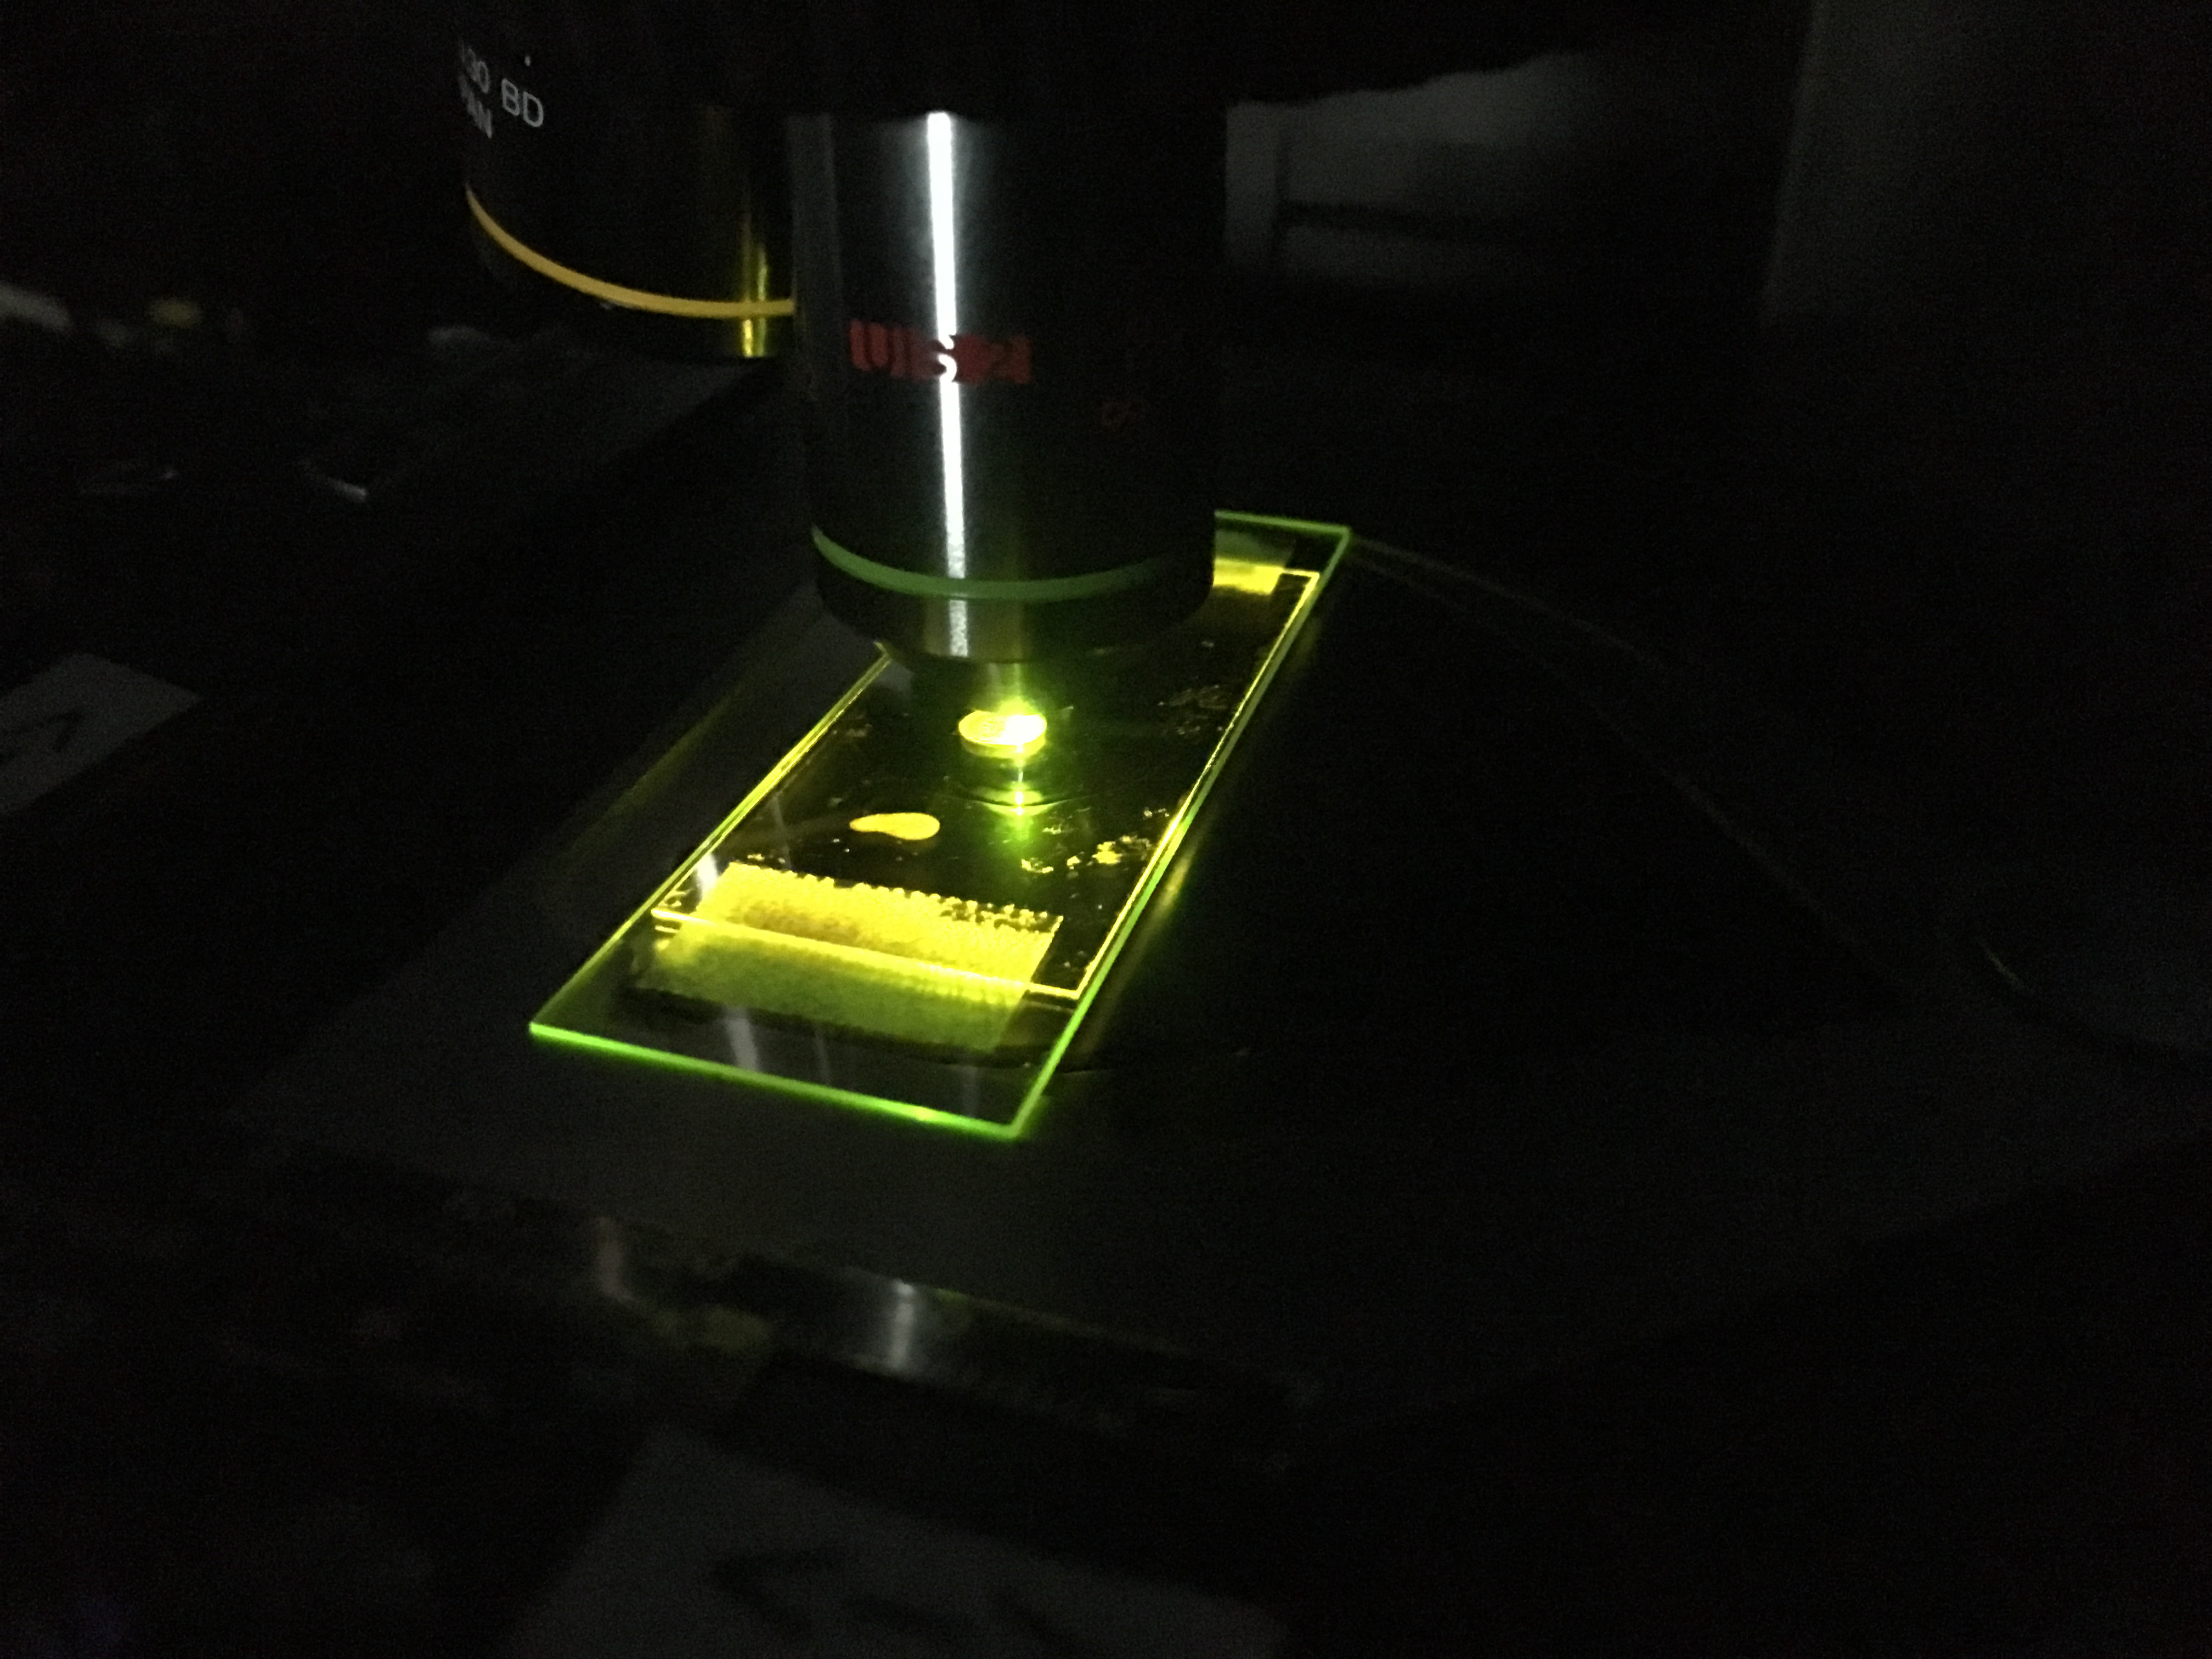
\includegraphics[width=0.75\textwidth]{img/objective-sample.JPG}
    \caption[Sample on stage under laser illumination.]{A sample of CdSe quantum dots under laser illumination at 405 nm. Some of the violet laser light is reflected by the sample, but is difficult to distinguish from the sample's intense green emission.}
    \label{img:objective-sample}
\end{figure}

We were able to fix a digital camera to the binocular optic for simple imaging of samples with adapters on hand. The camera is connected via USB to a desktop computer with software for capturing images. Example images are shown in Figures \ref{img:tesf} and \ref{img:qd}.


\subsection{Laser Alignment}
We aligned the laser to the microscope's optical axis by iteratively adjusting the two flat mirrors that direct the beam into the side of the microscope. First, we adjust the position of the beam as it enters the mirror cube housing by moving the first mirror. A reticle made of photoluminescent laser viewing material was a particularly useful target when fixed to the opening on the side of the mirror cube housing. 

We then adjust the second mirror in the beam fold to change the angle at which the beam is incident on the dichroic mirror. This translates the beam across the back of the microscope nosepiece, where our target is the optical axis of the objective lens. In place of a lens, we fix an iris diaphragm to the nosepiece. We adjust the second mirror to position the laser in the center of the mostly-closed iris, which marks the location of the optical axis of a lens. This process is repeated until the laser spot is centered on both targets.



  \section{Results and Discussion}
  In general, results from the microspectrometer are much smoother than results from the fluorimeter, which include quite a lot of noise. We suspect that this is a consequence of wide-field illumination used by the fluorimeter, in which molecules outside the region of interest (or otherwise, with some defects) are excited and emit spectra different from that of the region of interest. \todo{Instead of this, explore power dependence. Need sources. Have some questionably reliable data for the laser, no data for the Horiba. Can I get some generic data for Horiba to compare?}

\subsection{ADT TES-F}

\begin{figure}[h]
    \centering
    \begin{subfigure}[b]{0.45\textwidth}
        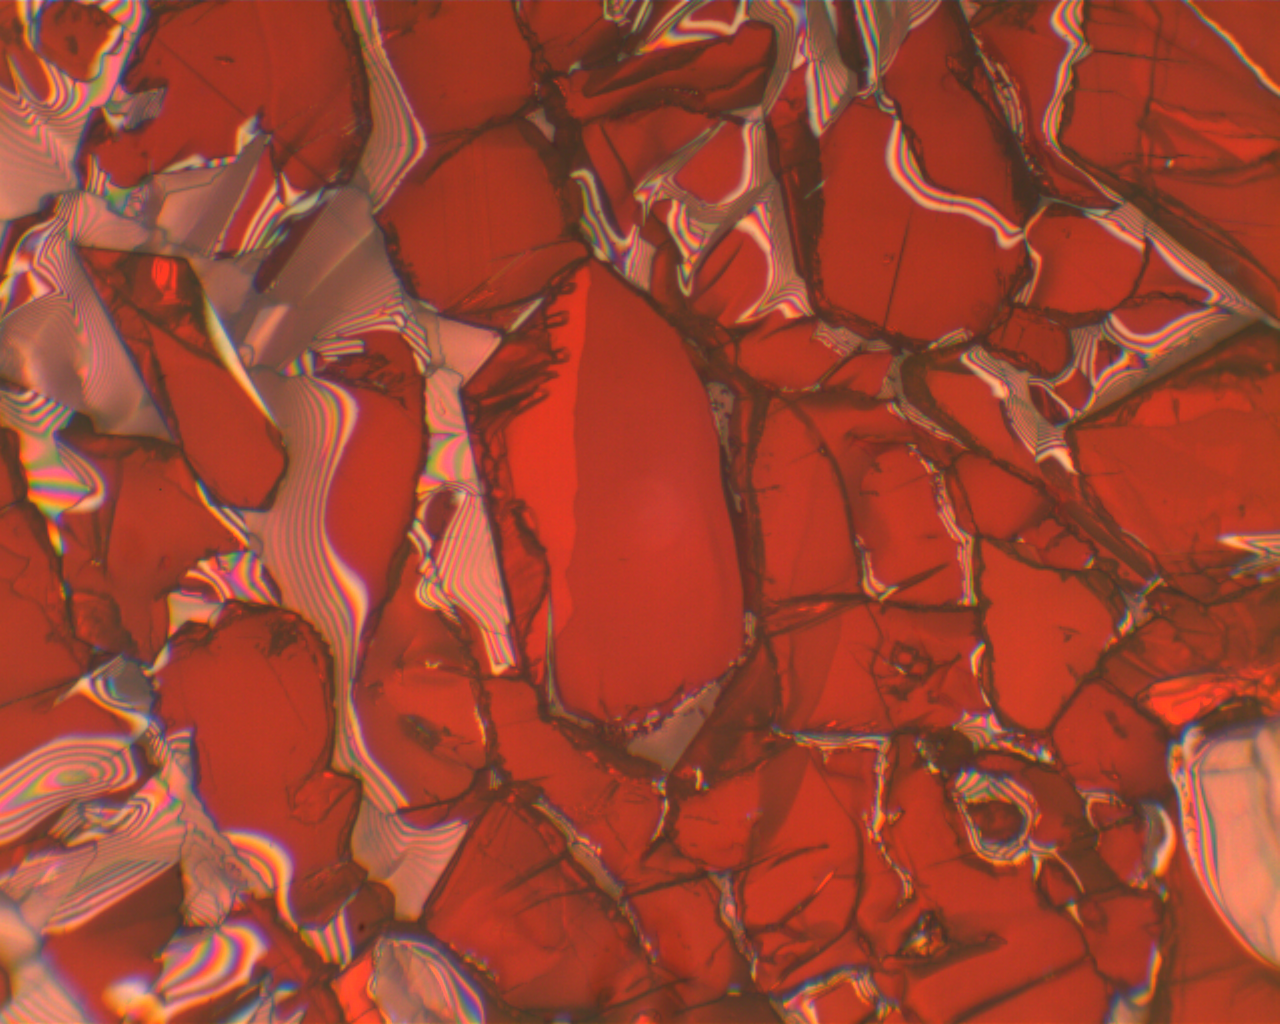
\includegraphics[width=\textwidth]{./img/tesf-white-illum.png}
        % \caption{TESF region of interest under white light.}
        \caption{}
        \label{img:tesf-white}
    \end{subfigure}
    \hfill
    \begin{subfigure}[b]{0.45\textwidth}
        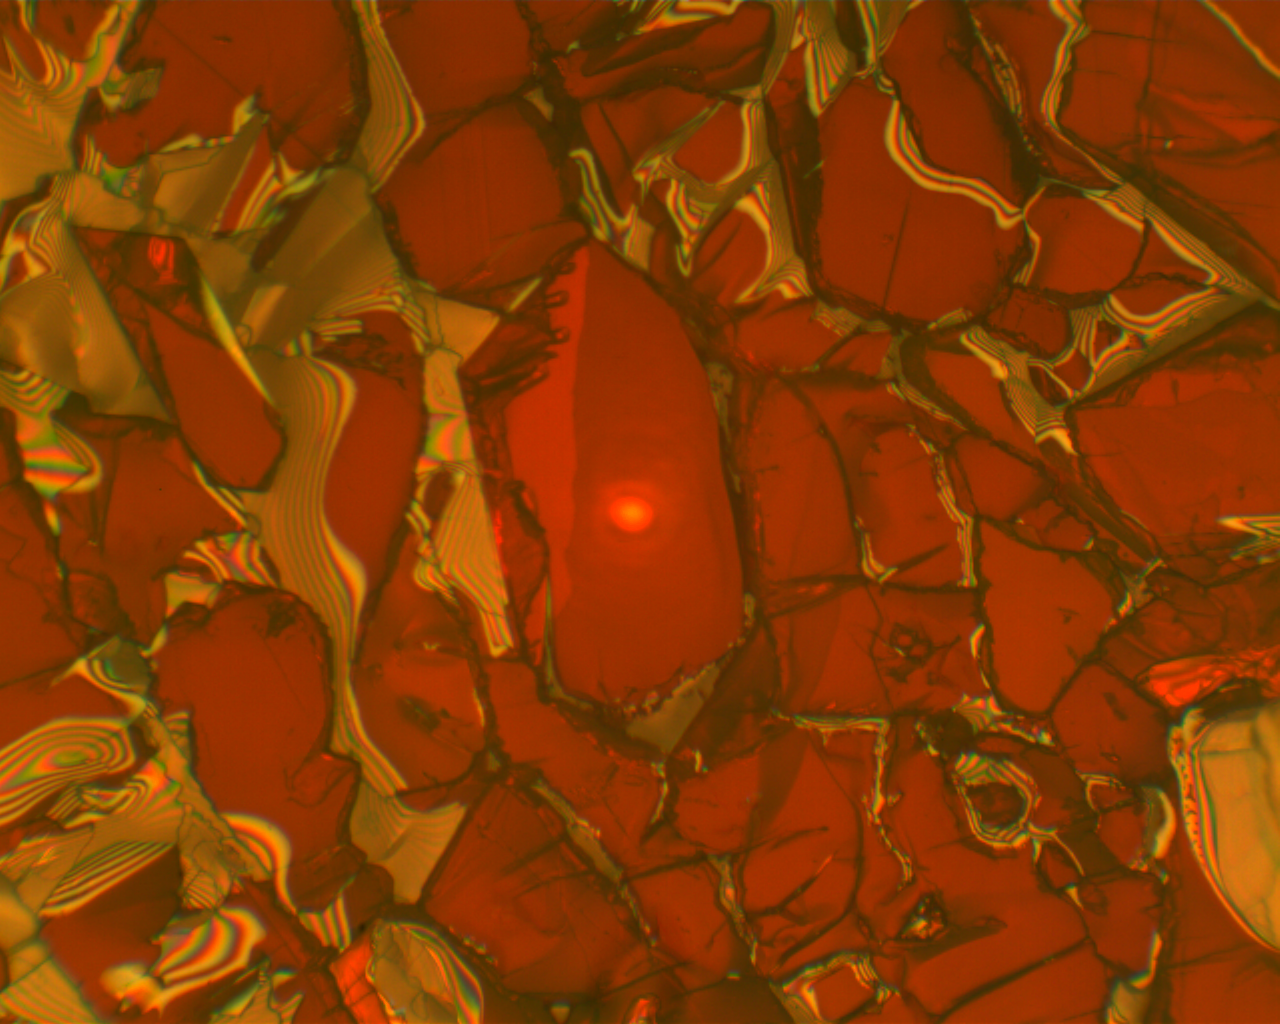
\includegraphics[width=\textwidth]{./img/tesf-laser-illum.png}
        % \caption{TESF region of interest under excitation light.}
        \caption{}
        \label{img:tesf-laser}
    \end{subfigure}
    \caption{Images of ADT TES-F sample under white light (\ref{img:tesf-white}) and under laser excitation light (\ref{img:tesf-laser}). Photoluminescence spectra of this region are shown in Figure \ref{fig:pl-adt-tesf}.}
    \label{img:tesf}
\end{figure}

For a drop-cast sample of ADT TES-F on glass, we selected a region of interest which appeared to be a single crystal, with few visually distinguishable defects (Figure \ref{img:tesf}). The crystal was also selected such that its surface area was larger than the area illuminated by the microspectrometer's laser spot. The emission spectra of the region of interest are shown in Figure \ref{fig:pl-adt-tesf}.

\todo{Convert wavelength from nm to eV? This seems to be a more common unit in solid state.}

Both spectra in Figure \ref{fig:pl-adt-tesf} show a clear peak around 630nm, which has been shown in other research.\cite{lam_polarization_2018}\cite{ostroverkhova_organic_2016}\cite{platt_optical_2009} The spectra measured by the microspectrometer also shows a secondary peak just below 600 nm, which is not evident in the spectrum taken by the fluorimeter. \note{All 3 citations in this paragraph have spectra with peaks similar to mine, but different intensity. This must be because they excited at a different wavelength, but how do I use that?}

\begin{figure}[h]
    \centering
    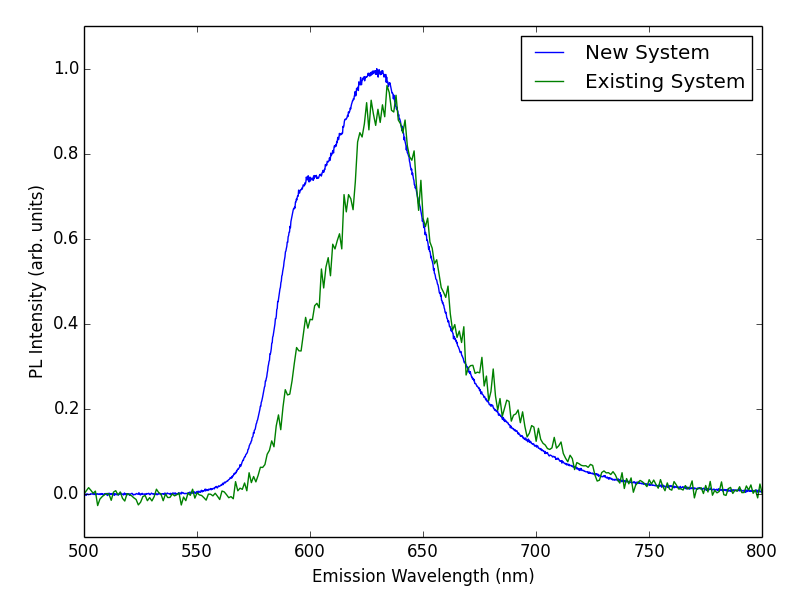
\includegraphics[width=.8\textwidth]{./img/tesf-2.png}%\llap{\raisebox{4cm}{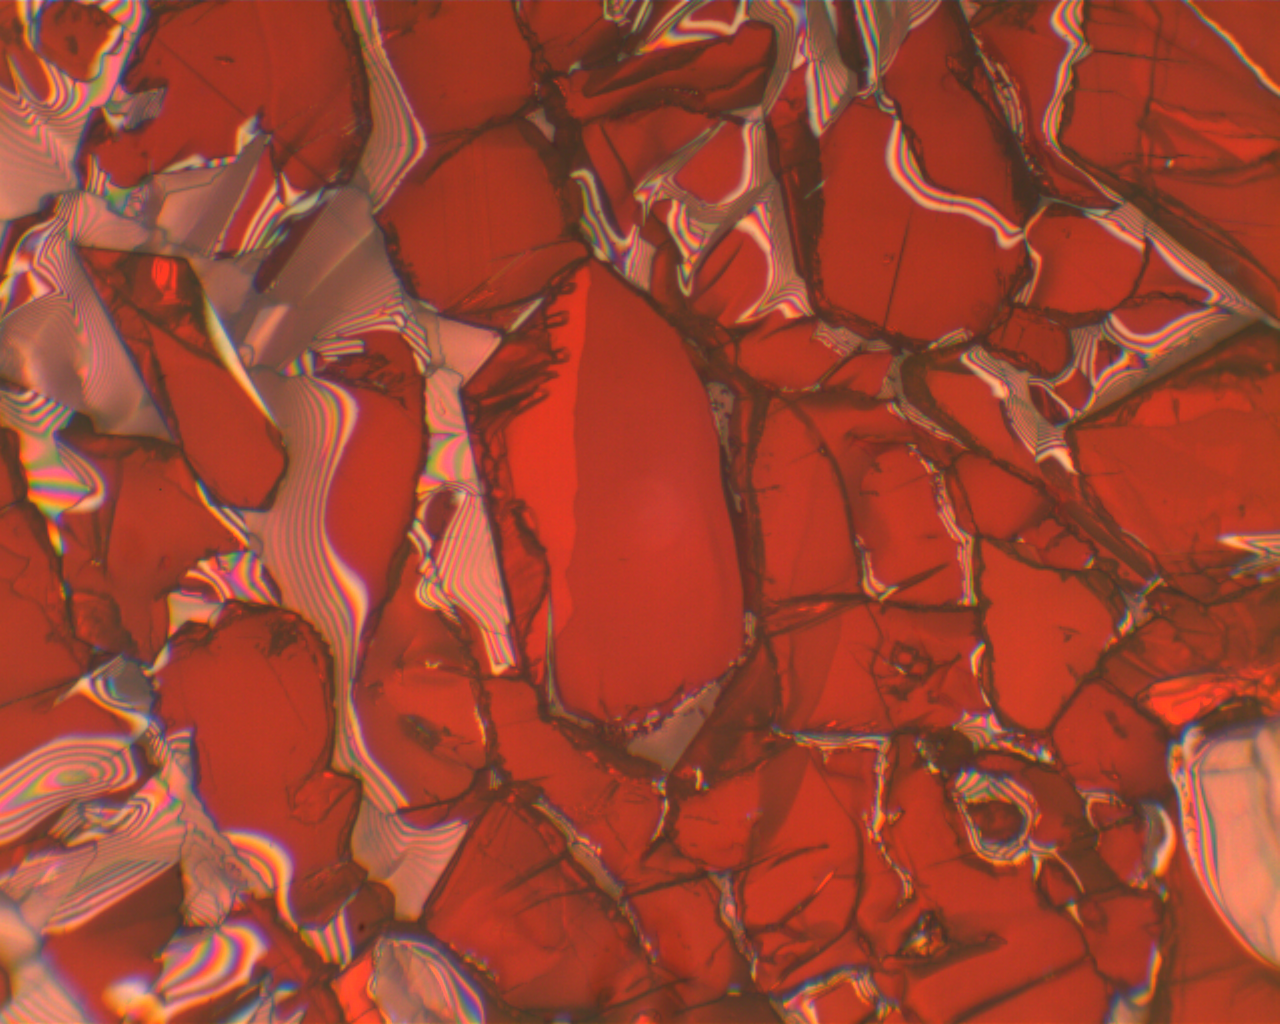
\includegraphics[width=2cm]{img/tesf-white-illum.png}}}
    % 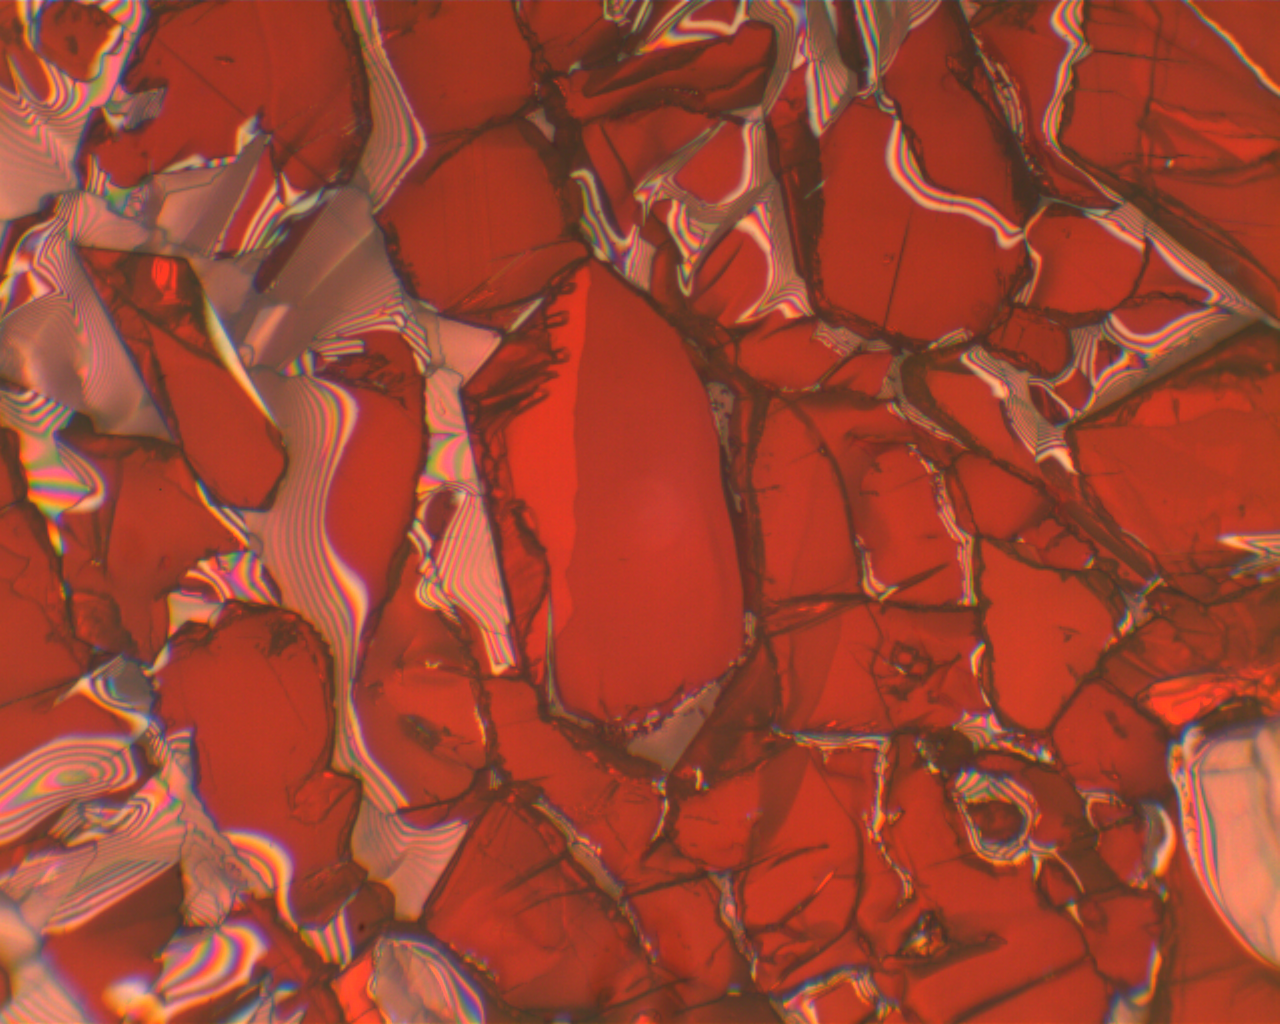
\includegraphics[width=.2\textwidth]{./img/tesf-white-illum.png}
    % 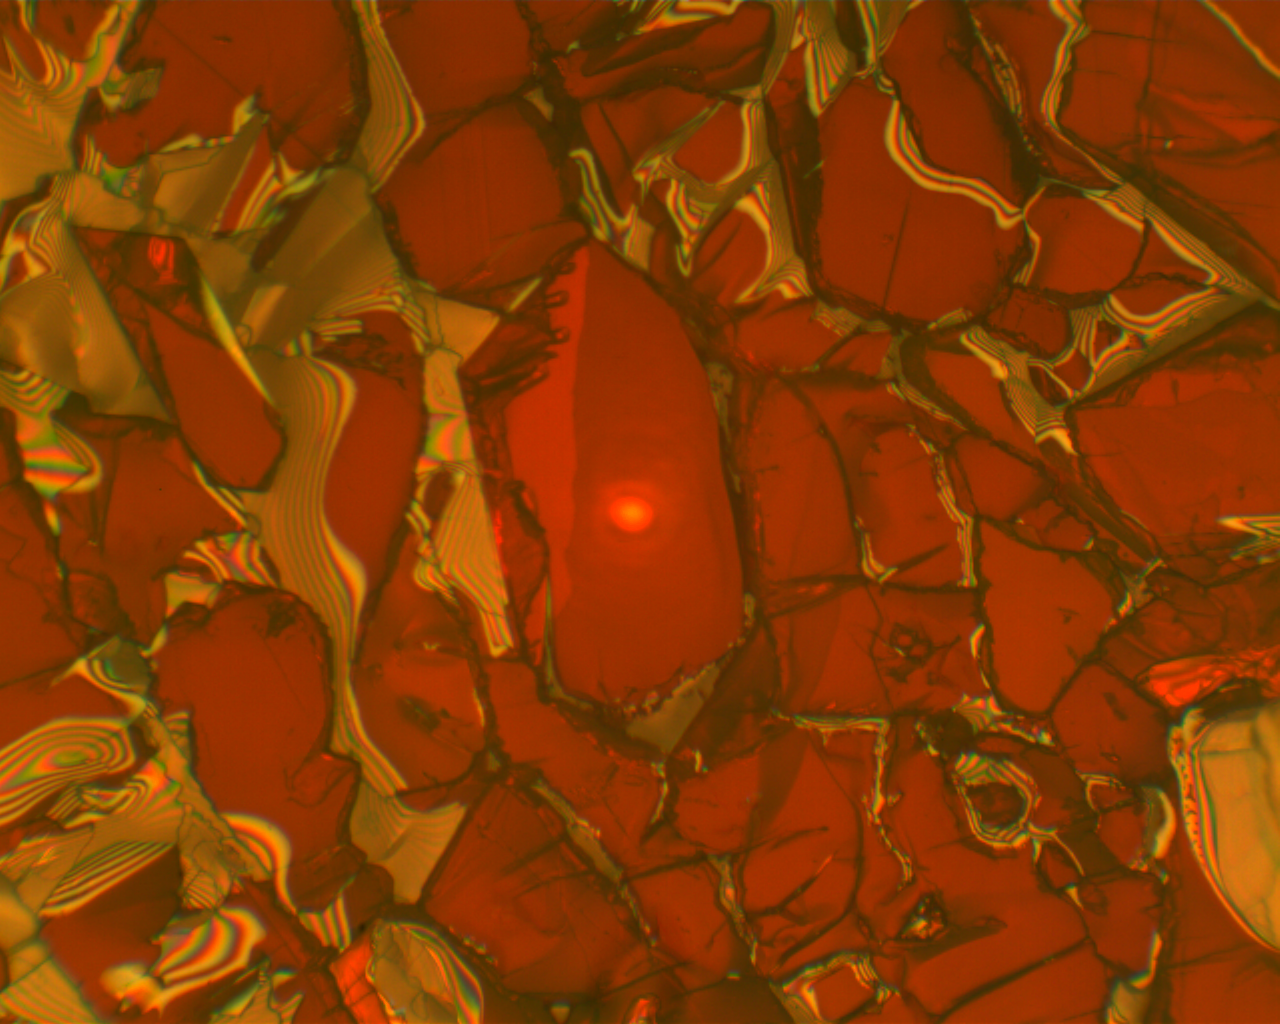
\includegraphics[width=.2\textwidth]{./img/tesf-laser-illum.png}
    \caption[PL emission spectrum of ADT TES-F, excited at 405nm.]{PL emission spectrum of ADT TES-F, excited at 405 nm.
    Wide-field illumination used by the existing system to excite the sample
    yields a noisy spectrum, and does not excite the secondary peak that is 
    shown clearly in the results from the new system. A single crystal, larger than the laser spot, was selected among smaller neighboring crystals for this measurement. %This may be because the
    %wide-field illumination is exciting many adjacent crystals in the sample, 
    %which emit slightly different spectra. The laser illumination in the new 
    %system has the spatial resolution necessary to illuminate single crystals.
    }
    \label{fig:pl-adt-tesf}
\end{figure}

\subsection{\ce{CdSe} Quantum Dots}

\begin{figure}[h]
    \centering
    \begin{subfigure}[b]{0.45\textwidth}
        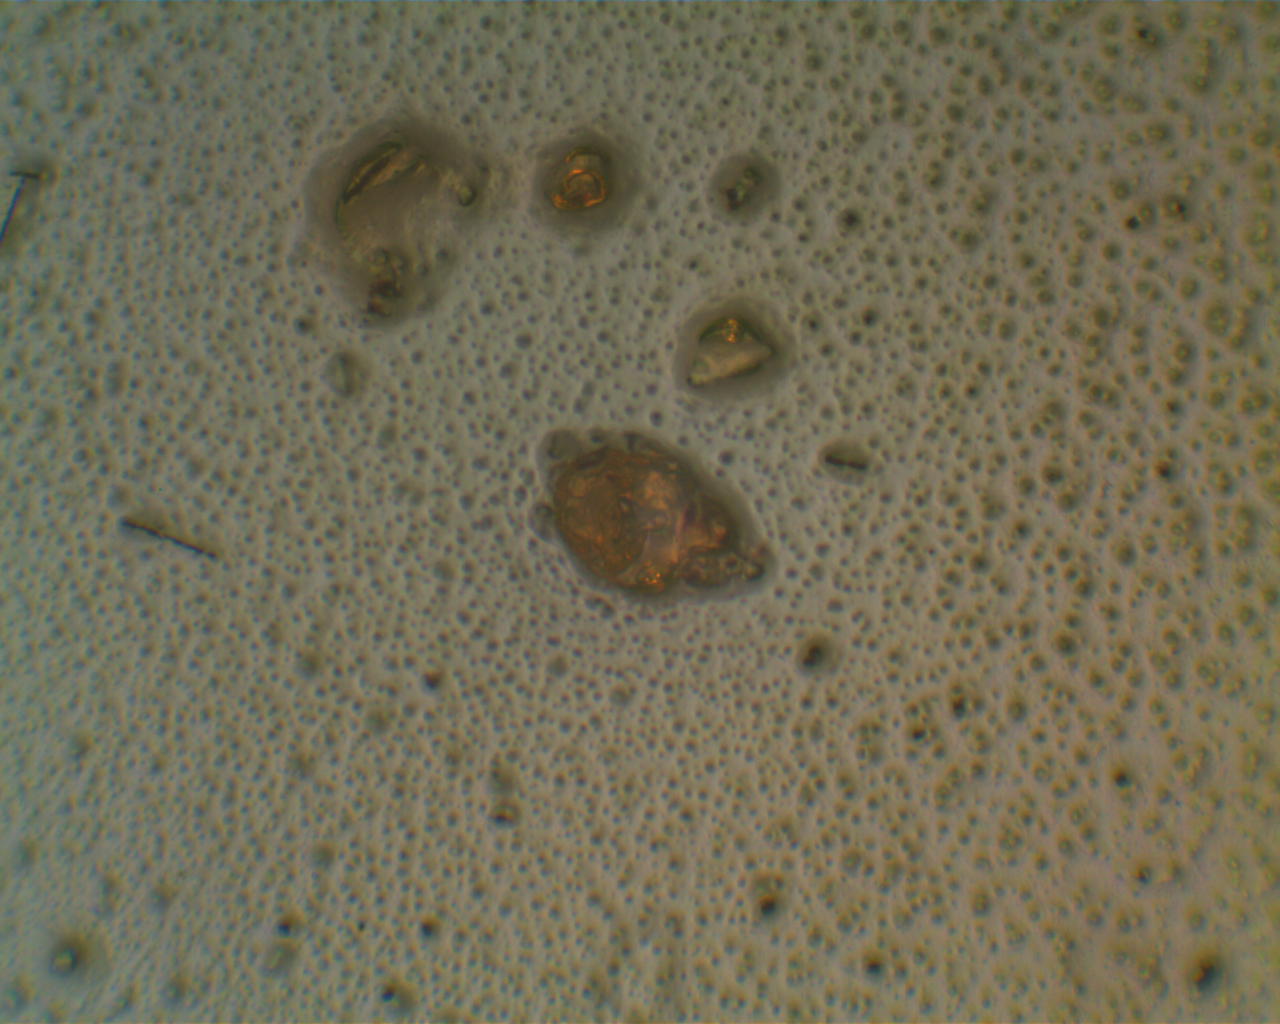
\includegraphics[width=\textwidth]{./img/qd-white-illum.png}
        \caption{}
        \label{img:qd-white}
    \end{subfigure}
    \hfill
    \begin{subfigure}[b]{0.45\textwidth}
        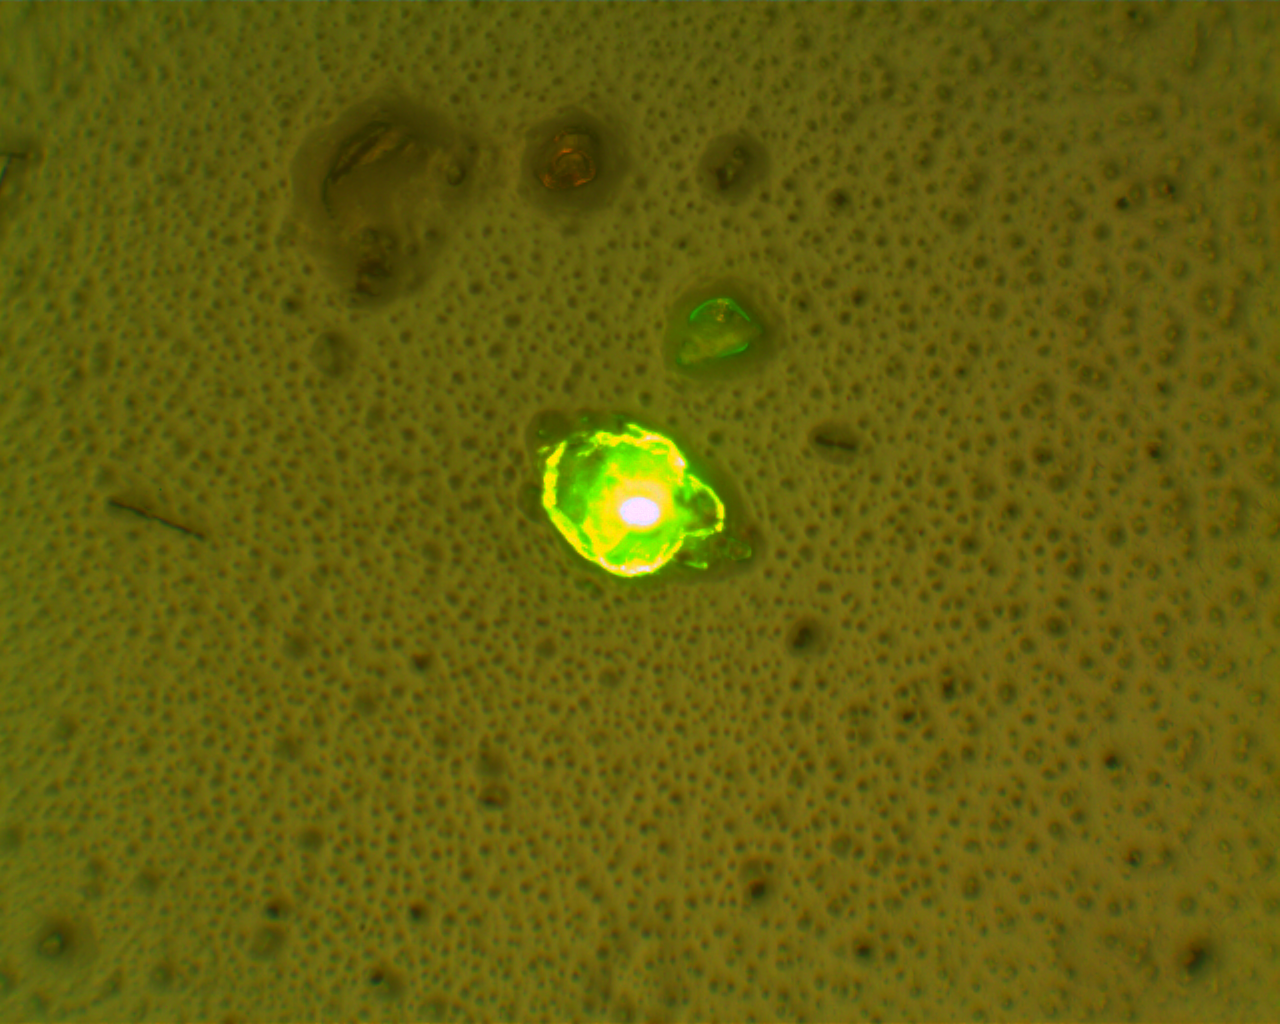
\includegraphics[width=\textwidth]{./img/qd-laser-illum.png}
        \caption{}
        \label{img:qd-laser}
    \end{subfigure}
    \caption{Images of CdSe quantum dot sample under white light (\ref{img:qd-white}) and under laser excitation light (\ref{img:qd-laser}). Photoluminescence spectra of this sample are shown in Figure \ref{fig:pl-adt-qd}.}
    \label{img:qd}
\end{figure}

Figure \ref{fig:pl-adt-qd} shows the PL emission of CdSe quantum dots \todo{on what substrate?}. There is one broad, clear peak that aligns well with the same measurement taken on the fluorimeter, between 520 and 620 nm. This peak seems to agree with other studies of CdSe quantum structures.\cite{empedocles_photoluminescence_1996}

Unlike the same measurement taken on ADT, this measurement was taken in a region of interest which is sparsely populated with quantum dots, with one target grouping illuminated by the laser.

\todo{What else do I write about here? Need to find more resources on analysis of PL, i.e. what information we get about the material. This will also be useful for Background section.}

\begin{figure}[h]
    \centering
    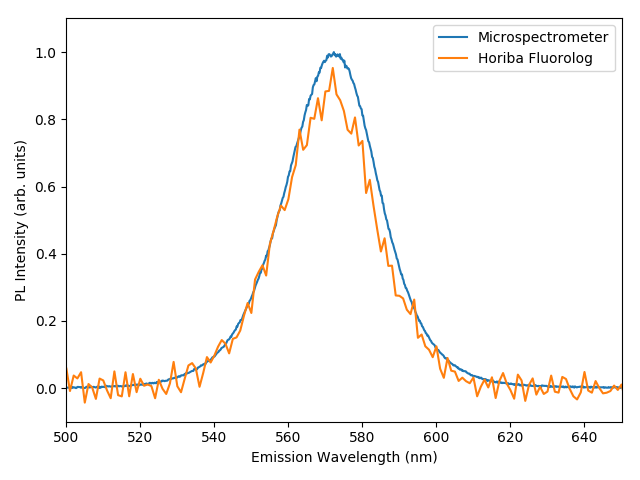
\includegraphics[width=\textwidth]{./img/qd-2.png}
    % 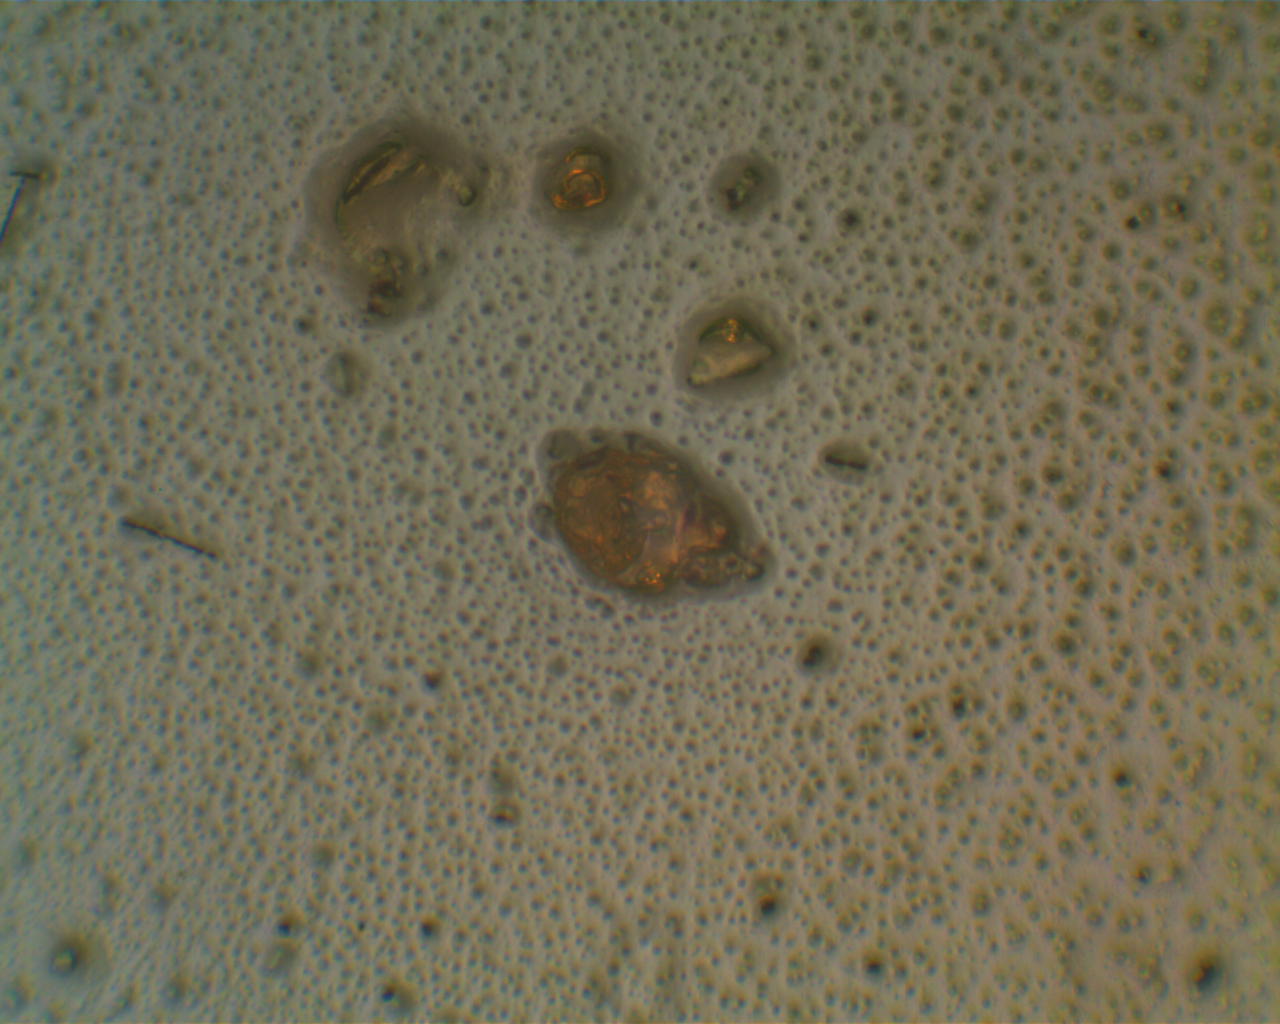
\includegraphics[width=4cm]{./img/qd-white-illum.png}
    % 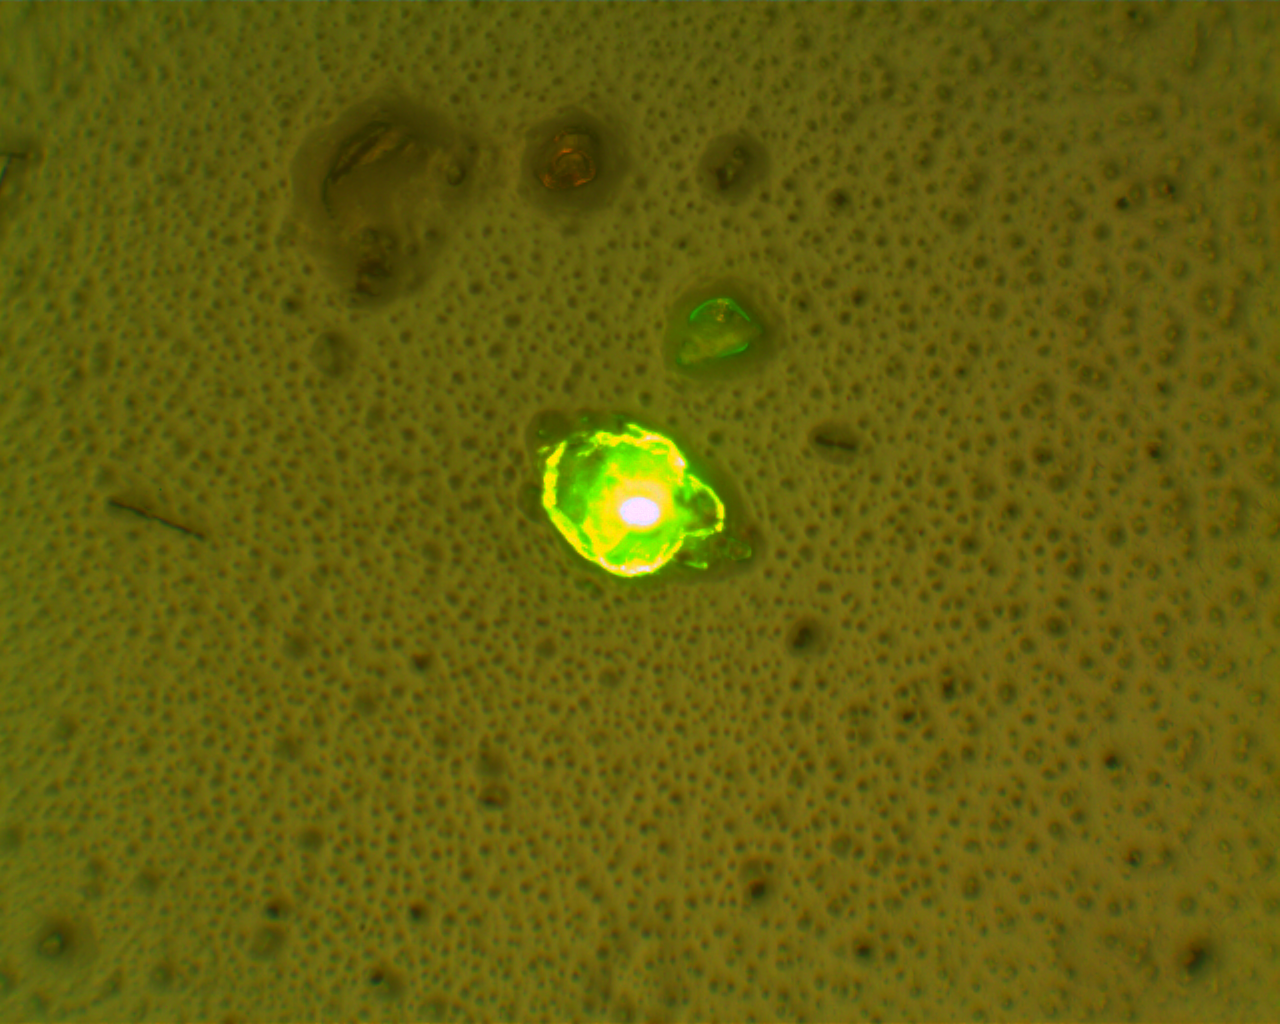
\includegraphics[width=4cm]{./img/qd-laser-illum.png}
    \caption{PL emission spectrum of a cluster of CdSe quantum dots on ?? substrate, excited at 405 nm.}
    \label{fig:pl-adt-qd}
\end{figure}


  \section{Conclusion}
  \todo{Conclusion}

  \section{Acknowledgements}
  % This is a test citation. \cite{edmund_optics_simplifying_nodate}
  \todo{Acknowledgements}
  
  \printbibliography[title=References]

%   \appendix
%   \section{Code}
%   \input(appendix/code)

\end{document}